\documentclass[12pt,fleqn]{article}\usepackage{../../common}
\begin{document}
Modern Bilim Önceki Bilimsel, Astronomik Buluşlar, Gezegenler, Yörüngeler

Dunya - Ay Mesafe Oranı

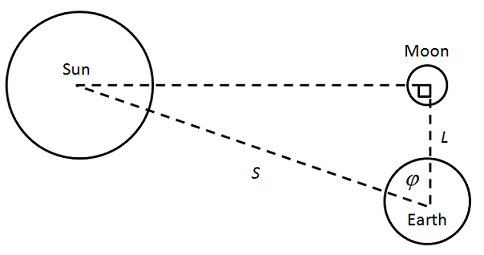
\includegraphics[width=20em]{sunmoon.png}

\begin{minted}[fontsize=\footnotesize]{python}
print (1./np.cos(np.deg2rad(87)))
\end{minted}

\begin{verbatim}
19.10732260929735
\end{verbatim}

Dünyanin Yuvarlaklığı, ve Çevre Uzunluğu

Eratosten (Erotosthenes) MO 276 - MO 194 yıllarında yaşayan bilim adamıdır,
İskenderiye kütüphanesinin başındaydı. Bir gün birinden öğrendi ki yazın en uzun
günü 21. Haziran'da daha güneyde olan Syene şehrinde eğer yere bir çubuk
dikilirse, saat 12'de çubuğun hiç gölgesi olmuyor. Pitagor zamanından beri
aslında dünyanin yuvarlak olabileceği düşünülüyordu, Eratosten acaba aynı uzun
yaz gününde daha kuzeyde olan İskendiriye'de yere bir çubuk dikersem saat 12'de
ne görürüm.

Bunu yaptı ve gördü ki ufak ta olsa bir gölge var. 

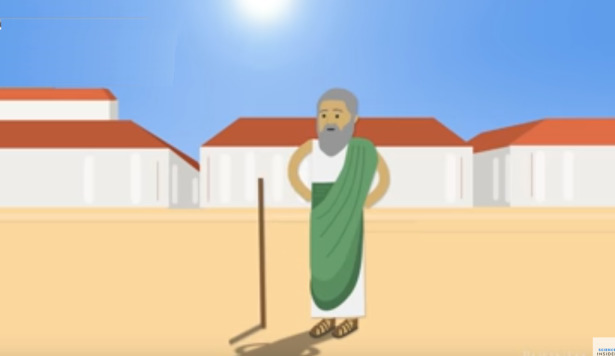
\includegraphics[width=20em]{circum3.jpg}

Sonra bu gölgenin sonuna kadar sopa basından doğru bir çizgi çekince, oluşan
açıya baktı,

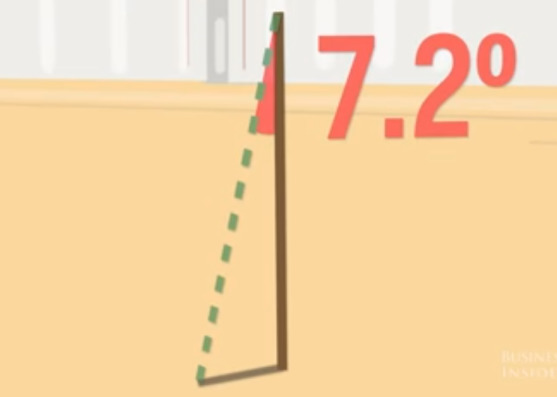
\includegraphics[width=20em]{circum4.jpg}

Bu önemli bir bilgiydi çünkü şimdi gökyüzüne düşen güneş ışınlarını düşünelim,
işin öyle düşüyor ki o açı oluşmuş, 

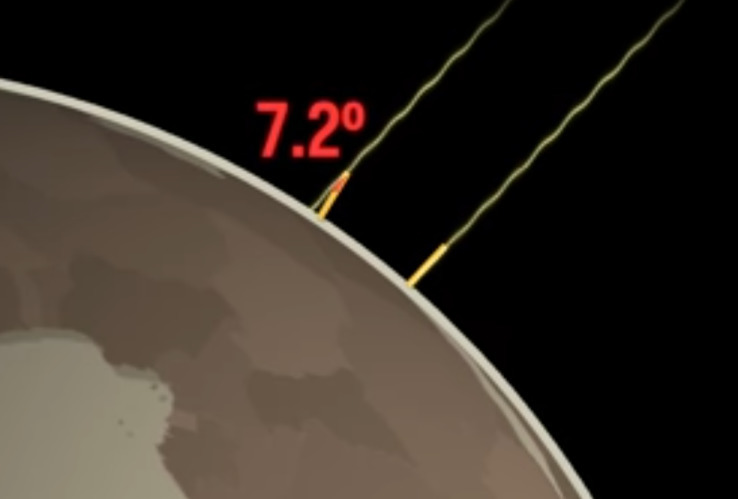
\includegraphics[width=20em]{circum1.jpg}

Şimdi bu ışını düz uzatırsak, bir de sopanın yönünde direk bir çizgiyi direk
dünya merkezine çekersek, bir üçgen ortaya çıkar, bir çizgiyi Syene şehrinin
sopasından direk dünya merkezine uzatabiliriz (bu çizgi direk merkeze gider
çünkü biliyoruz ki o anda oradaki sopanın gölgesi yok, güneş ışını direk sopanın
tepesine geliyor)

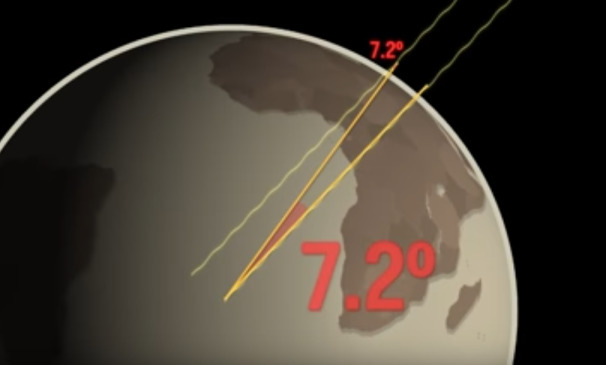
\includegraphics[width=20em]{circum2.jpg}



Kaynaklar

[1] Wikipedia,
    \url{https://en.wikipedia.org/wiki/On_the_Sizes_and_Distances_(Aristarchus)}

[2] Science Insider, {\em How The Ancient Greeks Proved Earth Wasn't Flat 2,200 Years Ago},
    \url{https://youtu.be/EfZ2HZH5CkA}
    
\end{document}
